
\documentclass[10pt]{exam}
\usepackage{graphicx}
\usepackage{listings}

\newcommand{\R}{\mathbb{R}}
\newcommand{\changes}[1]{{\color{red} #1}}
\usepackage{xcolor}
\usepackage[english]{babel}
\usepackage{amsmath,amssymb,amsthm,mathdots}
\usepackage{graphicx}
\usepackage[colorinlistoftodos]{todonotes}


\renewcommand{\thequestion}{\arabic{question} }
\renewcommand\questionlabel{\llap{\thequestion)}}


\usepackage{xcolor}
\definecolor{SolutionColor}{rgb}{0.1,0.3,1}

\unframedsolutions
\shadedsolutions
\definecolor{SolutionColor}{rgb}{0.9,0.9,1}
\renewcommand{\solutiontitle}{\textbf{Solution}$:\>$  }




%Mathcal and 
\newcommand{\mb}[1]{\mathbb{#1}}
\newcommand{\mc}[1]{\mathcal{#1}}

%Various possibilities for norms
\newcommand{\norm}[2]{\|#1\|_{#2}}
\newcommand{\normtwo}[1]{\|#1\|_{2}}
\newcommand{\normp}[1]{\|#1\|_{p}}

\newcommand{\rn}{\mathbb{R}^n}
\newcommand{\rnn}{\mathbb{R}^{n\times n}}
\newcommand{\rmn}{\mathbb{R}^{m\times n}}



%Boldface for vectors and tildes
\renewcommand{\vec}[1]{{#1}•}
\newcommand{\mat}[1]{{#1}•}

\newcommand{\vect}[1]{\widetilde{\boldsymbol{#1}}}
\newcommand{\matt}[1]{\widetilde{\boldsymbol{#1}}}

%Column and row equivalence
\newcommand{\roweq}{\stackrel{\text{row}}{\sim}}
\newcommand{\coleq}{\stackrel{\text{col}}{\sim}}

\newtheorem{definition}{Definition}
\newtheorem{example}{Example}
\newtheorem{fact}{Fact}
\newtheorem{remark}{Remark}


%Vector spaces
\newcommand{\rank}{\text{rank}\,}
\renewcommand{\dim}{\text{dim}\,}
\newcommand{\Span}[1]{\text{Span}\,\{#1\}}
\newcommand{\basis}[1]{\left\{ #1\right\}}


%Matrix environments
\newcommand{\bmat}[1]{\begin{bmatrix}#1\end{bmatrix}}
\newcommand{\pmat}[1]{\begin{pmatrix}#1\end{pmatrix}}
\newenvironment{amatrix}[1]{%
  \left(\begin{array}{@{}*{#1}{c}|c@{}}
}{%
  \end{array}\right)
}


%Trace and determinant
\newcommand{\diag}{\mathsf{diag}\,}
\newcommand{\range}{\mathsf{range}\,}
\newcommand{\trace}{\mathsf{trace}\,}


\usepackage{hyperref}
\title{MA 402: Project 4}
\author{Richard Watson, Mountain Chan, Cole Nash}
%\date{}
\begin{document}
\maketitle
\textbf{Instructions}: 

\begin{itemize}
\item Detailed instructions regarding submission are available on the class website\footnote{\url{https://github.ncsu.edu/asaibab/ma402/blob/master/project.md}}.
\item The zip file should contain three files hw4.pdf, hw4.tex, classnotes.sty. 

\end{itemize}

\vspace{2mm}

\begin{questions}

\question [10] The infamous RANDU generator was part of the Scientific Subroutine Package on IBM main-frame computers in the 1960s; the generator corresponds to
\[ I_{n+1} \equiv (a I_n + c) \text{mod} \> m, \qquad n = 0, 1, \dots \]
with $a = 65539$, $c = 0$ and $m = 2^{31}$.
\begin{parts}
\part  Show that  
\[ I_{n+2} - 6I_{n+1} + 9I_n \equiv 0 \> \text{mod} \> m. \]
{\em Hint}: Recall that $a \equiv b$ mod $m$ means $a = km + b$ for some integer $k$. Another useful fact is that $a = \changes{65539} = 2^{16} + 3$.

\begin{align*}
    I_{n+1} &= (aI_n)\text{ mod }m = (2^{16} + 3)I_n \text{ mod }m \\
    I_{n+2} &= (aI_{n+1}) \text{ mod }m = (2^{16} + 3)^2 I_n \text{ mod }m \\
    I_{n+2} - 6I_{n+1} +9I_n \text{ mod } m &= (2^{16} + 3)^2 I_n - 6(2^{16} + 3)I_n + 9I_n \text{ mod }m \\
    &= (2^{32} + 6 \cdot 2^{16} + 9)I_n - (6 \cdot 2^{16} + 18)I_n + 9I_n \text{ mod }m \\
    &= 2m I_n \text{ mod }m \\
    &\equiv 0\text{ mod }m
\end{align*}

Since the left side is obviously divisible by m we know that this is true.

\pagebreak

\part Implement RANDU and verify graphically its severe lack of equi-distribution by creating a three
dimensional plot of the $10,000$ points for some odd $I_0$ of your choice. More precisely, plot (in 3D)
\[ \{(I_{n-1},I_n,I_{n+1})/m\} \qquad n = 1,\dots,10,000.\]

At first glace it does look good and truly random.

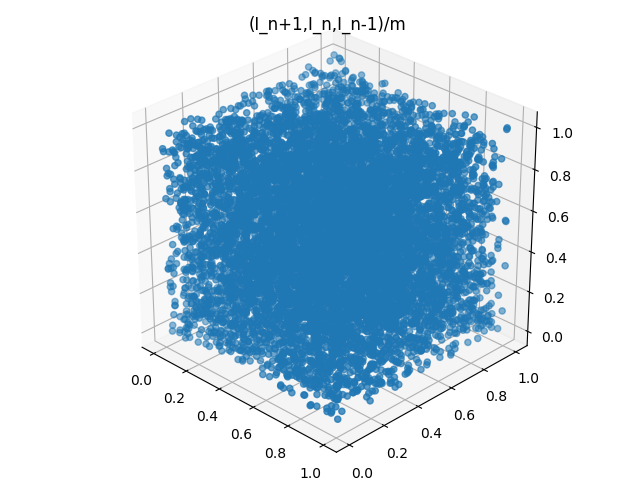
\includegraphics[scale = 0.5]{stilldumb.png}

But if you move it around a little you'll see,

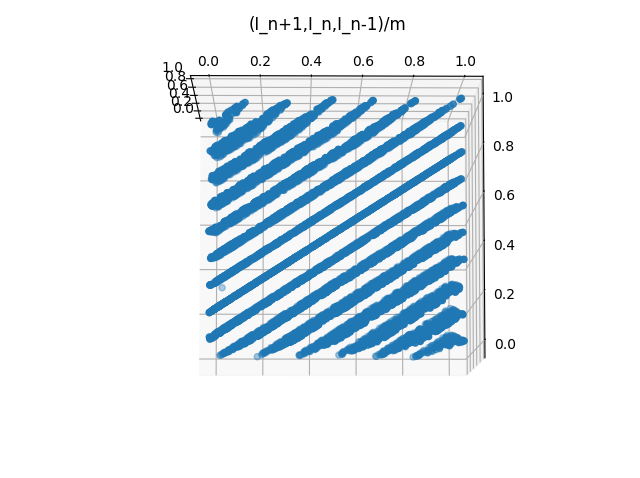
\includegraphics[scale = 0.5]{DUMBshit.png}

Which shows very clearly the lack of equi-distribution since they all clump together in defined planes.

\pagebreak

\part Plot $\{I_n/m\}$ for $n=1,\dots,10000$ as a histogram with $30$ bins.  

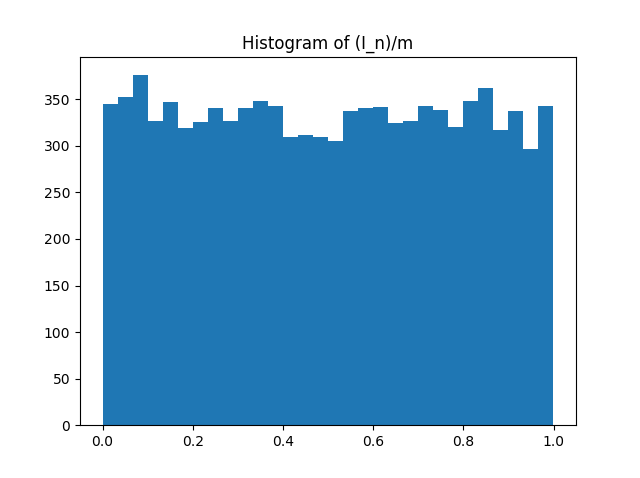
\includegraphics[scale = 0.5]{dumbhist.png}

This looks pretty normal.

\begin{lstlisting}[language = Python]
import pylab as py
import matplotlib.pyplot as plt
from mpl_toolkits.mplot3d import Axes3D

I_n = 126423 #totally arbitary
I = np.zeros(10000)
plotx = np.zeros(10000)
ploty = np.zeros(10000)
plotz = np.zeros(10000)
plot = np.zeros(10000)
I[0] = I_n
plot[0] = I_n / 2**31
plotx[0] = I_n / 2**31
ploty[1] = I_n / 2**31
plotz[2] = I_n / 2**31

for i in range(1, 10000):
    I[i] = ((65539.*I[i-1])%2**(31))
    plot[i] = I[i]/2**31
    plotx[i] = I[i]/2**31
    ploty[i-9999] = I[i]/2**31
    plotz[i-9998] = I[i]/2**31

#fig = plt.figure()
#ax = fig.add_subplot(111, projection='3d')
#ax.scatter( plotx, ploty, plotz, zdir='z')
#ax.set_title("(I_n+1,I_n,I_n-1)/m")

#f, ax = plt.subplots(1,1,sharey = True)
#ax.hist(plot, bins = 30)
#ax.set_title("Histogram of (I_n)/m")

plt.show()
\end{lstlisting}

\end{parts}

\pagebreak

\question [10] Certain Boeing 757 models are configured with $168$ economy seats. Experience shows that only $90\%$ of economy-class ticket holders actually show up to board the plane. If an airline sells $178$ tickets, then what is the probability of overbooking, so that some passengers do not get the seat they paid for? Compute using
\begin{parts}
\part  the Binomial distribution;  
\\
Let $X \sim Binomial(n = 178, p = 0.9)$, then everyone should get a seat when $X \leq 168$, \\ $P(X \leq 168) = 1- P(X = 169 \ldots 178) = 1 - \sum_{k = 168}^{178} {178 \choose k}(0.9)^k(0.1)^{178 - k} = 0.01325457318$
\part  the normal approximation to the Binomial distribution. 
\\
Using the normal distribution, $P(169 \leq X \leq 178) = P(\frac{168.5 - 178(0.9)}{\sqrt{178(0.9)(0.1)}} \leq Z \leq \frac{178.5-178(0.9)}{\sqrt{178(0.9)(0.1)}}) = P(2.07 \leq Z \leq 4.57) = 1 - 0.9808 = 0.0192$
\end{parts}
You may use MATLAB/Python scripts to compute the necessary quantities.


\question [15]  The county hospital is located at the center of a square whose sides are $3$ miles wide. If an accident occurs within this square, then the hospital sends out an ambulance. The road network is rectangular, so the travel distance from the hospital, whose coordinates are $(0, 0)$, to the point $(x_1, x_2)$ is $|x_1| + |x_2|$ (that is, the $1$-norm or the Manhattan distance). 
\begin{parts}
\part [10] If an accident occurs at a point that is uniformly distributed in the square, find the expected travel time of the ambulance.\\
\\
The area of the square is 36 miles, so $f(x_1,x_2) = \frac{1}{36}$ for $-3 \leq x_1,x_2 \leq 3$. Thus the expected travel distance is:
\begin{align*}
    E[|x_1|+|x_2|] &= \int_{-3}^3 \int_{-3}^3 (|x_1|+|x_2|)f(x_1,x_2) dx_1 dx_2\\
     &= \frac{4}{36} \int_{0}^3 \int_{0}^3 (x_1+x_2) dx_1 dx_2\\
     &= \frac{1}{9} \int_{0}^3 (\frac{9}{2}+3x_2)  dx_2\\
     &= \frac{1}{9} (\frac{27}{2}+\frac{27}{2})\\
     &= 3
\end{align*}
\part [5]  Compute this expectation using Monte Carlo integration. Report the results using $10,100,500$ samples.
\begin{lstlisting}[language = Python]
import numpy as np

def problem3(samples):
  total = 0
  for i in range(samples):
    x1, x2 = np.random.uniform(-3,3,2)
    total += abs(x1) + abs(x2)
  return total / samples
  
np.random.seed(42)
print([problem3(10),problem3(100),problem3(500)])
\end{lstlisting}
This gives us 3.25 for 10 samples, 3.10 for 100 samples, and 3.07 for 500 samples.
\end{parts}

\question [15] Many people believe that the daily change of price of a company’s stock on the stock market is a random variable with mean $0$ and variance $\sigma^2$ . That is, if $Y_n$ represents the price of the stock on the $n$th day, then
\[ Y_n  = Y_{n-1} + X_n \qquad n\geq 1\]
where $X_1,X_2,\dots$ are independent and identically distributed random variables with mean $0$ and variance $\sigma^2$. Suppose that the stock's price today is $100$ and assume $\sigma^2 = 1$. 
\begin{parts}

\part Plot $20$ different trajectories of the stock prices over the next $10$ days.
\begin{lstlisting}[language = Python]
import numpy as np
import matplotlib.pyplot as plt

def problem4a(initial_price, n):
  arr = np.zeros([n+1])
  arr[0] = initial_price
  arr[1:] = np.random.normal(0,1,n)
  return np.cumsum(arr)
  
np.random.seed(42)

_, ax = plt.subplots(1,1)
for i in range(20):
  ax.plot(problem4a(100,10))
  
ax.set_xlabel('Nth Day')
ax.set_ylabel('Price')
ax.set_title('20 Stock Price Trajectories for 10 Days')
  
plt.show()
\end{lstlisting}
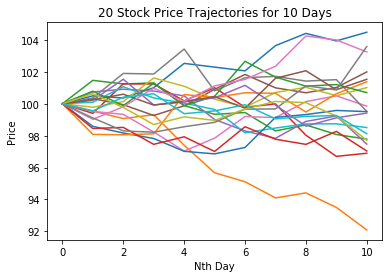
\includegraphics[]{TooEazy.png}

\part Using Monte Carlo, estimate  the  probability that the stock’s price will exceed $105$ after $10$ days. Report the results using $10,100,500$ samples. \\

{\em Hint:} Let $X = Y_{10} =  Y_0 + \sum_{i=1}^{10} X_i$. Use the fact that $P(X \geq 105) = E[I_{X \geq 105}]$, where $I_{X \geq 105}$ is an indicator random variable
\[ I_{X \geq 105} = \left\{ \begin{array}{ll} 1 & X \geq 105 \\ 0 &  \text{otherwise}\end{array}\right. .\] 
\begin{lstlisting}[language = Python]
import numpy as np

def problem4b(initial_price, samples):
  arr = np.ones([samples])*initial_price
  arr += np.sum(np.random.normal(0,1,size=(samples,10)),axis=1)
  return np.sum(arr >= 105)/samples
  
np.random.seed(42)
print([problem4b(100,10),problem4b(100,100),problem4b(100,500)])
\end{lstlisting}
This gives us 0.0 for 10 samples, 0.06 for 100 samples, and 0.038 for 500 samples.

\part Compute this probability analytically. You can use the fact that if $X_i$'s are independent normal random variables with mean $\mu$ and variance $\sigma^2$, then $\sum_{i=1}^n X_i$ is also a normal distribution with mean $n\mu$ and variance $n\sigma^2$.
\begin{align*}
    P(X \geq 105) &= P(Y_{10} \geq 105)\\
     &= P(Y_0 + \sum_{i=1}^{10} X_i \geq 105)\\
     &= P(100 + \sum_{i=1}^{10} X_i \geq 105)\\
     &= P(\sum_{i=1}^{10} X_i \geq 5)\\
     &= 1 - P(\sum_{i=1}^{10} X_i < 5)\\
     &= 1 - P(\frac{5 - 0}{\sqrt{10}} < z)\\
     &= 1 - 0.9429\\
     &= 0.0571
\end{align*}

\end{parts}

\end{questions}

\end{document}




